%!TEX root = ../main.tex
%%%%%%%%%%%%%%%%%%%%%%%%%%%%%%%%%%
% Links:
%
% Difficulty: Companies: 
%%%%%%%%%%%%%%%%%%%%%%%%%%%%%%%%%%

\chapter{Count the number of islands}
\label{ch:number_islands}
In this chapter we are going to discuss a classical interview problem question. The problem asks you
to count the number islands on a map that is given to you as a 2D boolean matrix. There are many
version of the statements for this problem, some with for instance more wordy and playful background
story and others where the map is given to you as graph of some sort. Thankfully all of those
versions can be solved with the approaches we will present below. The solutions presented are based
on textbook graph visiting algorithms.

\section{Problem statement}
\begin{exercise}
Write a function that given a $2$D boolean matrix counts the number of islands in the grid. Cells in
the input matrix containing a $1$ represent land while $0$  water. An island is a group of adjacent
land cells. Every cell in the input matrix can be adjacent to the $4$ cells that are next to it on
the same row or column.

The input grid is a 2D \inline{std::vector<std::vector<bool>>} of size $n\times m$. 
	\begin{example}
		\hfill \\
		Given the following input grid (depicted in Figure \ref{fig:number_islands:example1}) the
		function return $4$. The text representation of this example is given below where $1$
		represents land, and a $0$ water:	
	\begin{verbatim}
	1110000
	0100000
	0110110
	0010110
	0100000
	0110010
	0011000
	\end{verbatim}
	\end{example}

\end{exercise}

\begin{figure}
	\centering
	\begin{subfigure}[t]{0.45\textwidth}
		\centering
		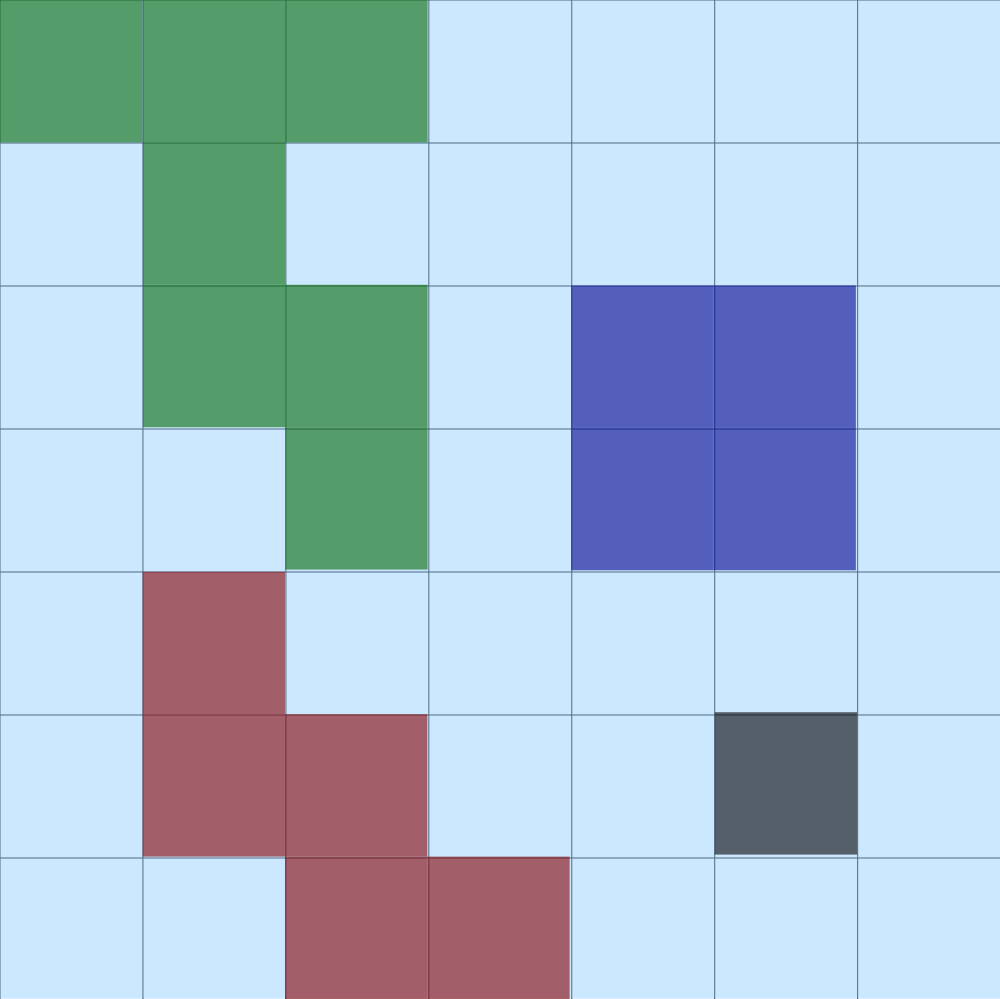
\includegraphics[width=\textwidth]{sources/number_islands/images/example1}
		\caption{Visual representation of the example 1 for the problem of counting the number of islands in a map. Cells belonging to the same island share the same color.}
		\label{fig:number_islands:example1}
	\end{subfigure}
	\hfill
	\begin{subfigure}[t]{0.45\textwidth}
		\centering
		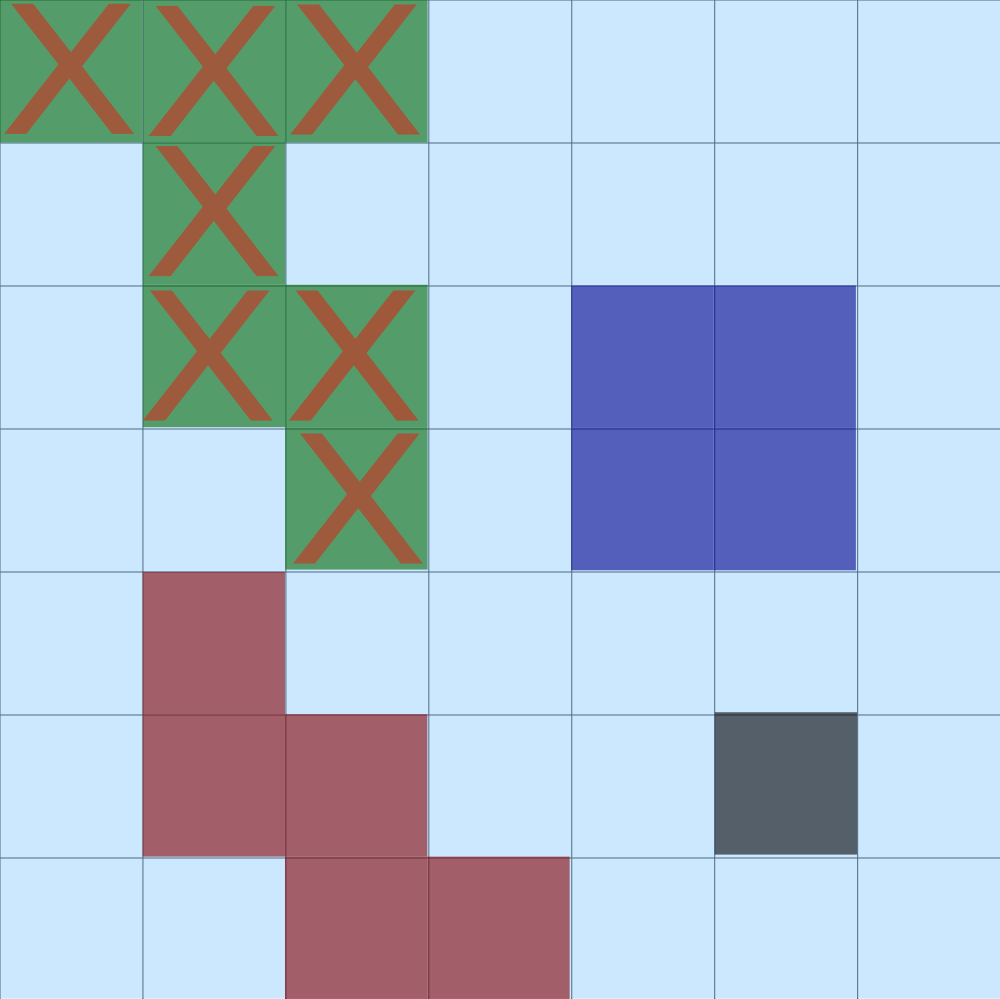
\includegraphics[width=\textwidth]{sources/number_islands/images/visited}
		\caption{Visual representation of the example 1 after visiting the cells of the first island.}
		\label{fig:number_islands:example1_visited}
	\end{subfigure}
\end{figure}

\section{Clarification Questions}

\begin{QandA}
	\item Can $n$ or $m$ be $0$?
	\begin{answered}
		\textit{Yes, the map can be empty}
	\end{answered}
	\item Can the input grid be modified?
	\begin{answered}
		\textit{Yes, the input matrix is not read-only.}
	\end{answered}
\end{QandA}

\section{Discussion}
\label{number_islands:sec:discussion}
In simple words what this problem is asking us is  to identify the numbers of  clusters of $1$s in the input matrix.
One way to do so is by looping thought the map one cell at a time until we find a $1$, let's say at cell $(i,j)$.
Because this particular $1$ must be part of an island, then what we can do is to start exploring the island
one cell at a time, moving from a $1$ to an adjacent one, until there is no more $1$s we have not already visited.
When we visit a land cell we mark it as "visited".
This will be useful because, when we resume our normal linear scanning of the map, we want to make
sure we do not count the visited cells as being the starting point of an uncounted island.
For instance w.r.t. the example in Figure \ref{fig:number_islands:example1} we can start our visit
at cell $(0,0)$ which is a $1$ and it is not visited yet. This means that this particular cell is
part of a island that we did not count yet. At this point we can start visiting the cells adjacent
to $(0,0)$ i.e. cells: $(0,0), (0,1), (0,2), (1,1), (2,1), (2,2), (3,2)$. When a cell is visited is
marked as shown in Figure  \ref{fig:number_islands:visited} by the red cross
\textcolor[HTML]{860000}{$\times$} and after all of its neighboring land cell are visited similarly in a recursive manner.
When we have exhausted all the cells of the island $(0,0)$ is part of, we can resume our linear search remembering we have explored an additional island.

The visit can be performed using a BFS or DFS approach. In the following section we will shown a
recursive and iterative implementation of the DFS approach. We prefer the DFS approach to the BSF mostly because it is easier to 
code recursively.
The iterative version (in Listing \ref{sec:num_island:recursive}) however, can be turned
into a BFS quite easily by just changing the policy of the order with which cells are decided to be visited.


\subsubsection{DFS iterative}
\label{sec:num_island:iterative}
Listing \ref{list:number_islands:iterative} shows a possible iterative implementation of the DFS
approach described above. Note that the core of the algorithm is the function \inline{visit} that
uses a stack to keep track of the cells that are still to be visited. For each cell that is actually
visited we will also try to visit all pieces of yet unvisited land in all four directions (up, down,
left and right). We do so by adding them to the pile of cells to be visited. When a cell is actually
visited, it is marked as so in its corresponding cell of the array \inline{visited}.
When there is no  more land left in the stack it means that the island has been completely visited 
and we can return. Once it complete its execution the function \inline{visit}
returns the control back in the double loop of the function \inline{count_island_iterative_DFS} which will skip all the
visited cells and we will trigger another invocation of \inline{visit} as soon as another unvisited $1$ cell is
found. That $1$ has to be part of a not yet unaccounted island together with all its adjacents land cells.

Also please note how the if at line $22$ takes care of not visiting cells that are outside the
boundaries of the map, cells that are not land or already visited because this would lead to
out-of-bound errors, incorrect results and infinite loops, respectively.

The complexity of this implementation in Listing \ref{list:number_islands:iterative} is 
$O(n\times m)$ for both time and space 
because we visit the whole map at least once and we use space proportional to $n\times m$
for the array \inline{visited}.

\lstinputlisting[language=c++, caption={Iterative DFS solution to the problem of counting the number of islands in a map.},label=list:number_islands:iterative]{sources/number_islands/number_islands_solution1.cpp}

But, do we really need to have a dedicated matrix just to store the information about which cell is visited?
Turns out that we can store that information in-place in the input matrix. All is necessary, when marking a cell visited, is turning
the value in the input grid (which is modifiable) for that cell from land ($1$) to water ($0$) and that cell will never be considered part
of an island in the future. If we do that, the space complexity does not change because we still use
space to store the cells to be visited in the stack,
but the amount of space used will be lower in practice and the overall solution will look cleaner and simpler which is always a plus during an
interview. 

\lstinputlisting[language=c++, caption={Alternative iterative DFS solution, without dedicated space for marking visited cells,  to the problem of counting the number of islands in a map.},label=list:number_islands:iterative_1]{sources/number_islands/number_islands_solution2.cpp}

\subsubsection{DFS recursive}
\label{sec:num_island:recursive}
The same idea can also be implemented recursively. In our opinion doing it this way makes the
overall implementation more expressive, shorter and easier to reason about as well as to explain. Our first choice is always 
use this approach if possible when dealing with problem similar to the one presented here.
Listing \ref{list:number_islands:recursive} shows a possible implementation of a recursive DFS solution for
this problem. 
Notice that the recursion only happens during the DFS itself and that the driver
function \inline{count_island_recursive_DFS} is basically the same as the ones we showed in the
previous two solutions \ref{list:number_islands:iterative} and
\ref{list:number_islands:iterative_1}.

\lstinputlisting[language=c++, caption={Recursive DFS solution, to the problem of counting the number of islands in a map.},label=list:number_islands:recursive]{sources/number_islands/number_islands_solution3.cpp}